\documentclass{book}
\usepackage{graphicx}
\usepackage{amsmath}
\usepackage{float}
\usepackage{anyfontsize}
\usepackage[affil-it]{authblk}
\usepackage{fullpage}

\begin{document}

\author{Robert M. Johnson \\ rmj49@georgetotwn.edu}
\affil{ICBI \\ 2115 Wisconsin Ave NW, Suite 110}
\date{July 2014}



\begin{titlepage}
\begin{center}

% Upper part of the page. The '~' is needed because \\
% only works if a paragraph has started.
{\fontsize{50}{150}\selectfont The medTurk Book}

\includegraphics[scale=0.7]{../ui/img/medkit.png}~  \\[1cm]
July 14, 2014
\end{center}
\end{titlepage}


\frontmatter


\chapter*{Preface}
ICBI at Georgetown University is proud to provide this simple, yet effective, tool for converting unstructured clinical notes into structured data for clinical research. This book contains instructions on what medTurk is, how to use it, and how to set it up.
\\
\\
- Robert M. Johnson (rmj49@georgetown.edu)

\tableofcontents

\mainmatter

\chapter{Introduction}
medTurk is web application that coordinates the ingenuity of humans to convert unstructured clinical notes into structured clinical data for research. medTurk assumes there are clinical research questions of interest that could be answered by reading patients' clinical notes. medTurk organizes these questions and their allowed answers, in what's called a Research Model (RM). RMs can can organize answers .

medTurk uses a Research Model (RM) to encapsulate the questions you want answered, allowable answers (i.e. control fields), and a 'trigger' that identfies phrases in clinical notes that probably contain the answer to the question sought.

To organize these questions and allowed answers, medTurk uses 'Research Models' or RMs for short. A RM is a simple JSON file that organizes questions, answers, and taxonomies.

medTurk allows multiple users at once to answer questions and the project status page reports the percantage of project complete. The following chapter guides the installation process. Chapter 3 gives instructions on how to setup your first project.


\chapter{Installation}
In this chaper we guide you through the process of setting up medTurk. medTurk depends on Python and several Python packages. In addition, it requires cTAKES for processing clinical notes, a local running instance of UMLS, and a local running instance of MongoDB. This chapter instructs you on how to setup each of these components. We begin with Python's dependencies.

\section{Python}
medTurk requires a Python version of at least 2.7.6. On a Mac Terminal, you can use following line to retrieve the current Python version:
\begin{verbatim}
python --version
\end{verbatim}
Next, using pip, you must install the following Python packages:
\begin{verbatim}
pip install Flask
pip install mimerender
\end{verbatim}


\section{UMLS}
medTurk uses UMLS to look up names associated with CUIs reported by cTAKES. The following webpage provides instructions on how to setup a local UMLS MySQL database:

\begin{verbatim}
http://groups.csail.mit.edu/medg/projects/text/Load_UMLS_mysql.html
\end{verbatim}

\section{cTAKES}
Install cTAKES by following the instructions provided here:

\begin{verbatim}
https://cwiki.apache.org/confluence/display/CTAKES/cTAKES+3.1+User+Install+Guide
\end{verbatim}





\section{mongoDB}
Install mongoDB by following the instructions provided here:

\begin{verbatim}
http://www.mongodb.org/downloads
\end{verbatim}


\chapter{Creating Your First Project}

\section{Data Preparation}
medTurk requires patients' clinical notes to be in JSON format. Each JSON file should correspond to one patient. The name of the file is unimportant. Sample patient files can be viewed at:

\begin{verbatim}
https://github.com/ICBI/medkitpy/sample/patients/
\end{verbatim}

For convenience, we provide a snippet of one file here:
\begin{verbatim}
{
   "id":"5739",
   "records":[
      {
         "id":"1",
         "date":"2011-6-19",
         "note":"Jim is a 10 year-old male with newly diagnosed 
		   T-cell acute lymphoblastic leukemia diagnosed 5/26/2011. 
		   He is being treated according to COG protocol AALL0434 
		  (On Study) and is day 22 of Induction chemotherapy. 
		   Coming for follow-up and chemotherapy."
      },
      {
         "id":"2",
         "date":"2011-11-01",
         "note":"Jim is a 10 year-old male with newly diagnosed T-cell acute 
 		   lymphoblastic leukemia diagnosed 5/26/2011. 
		   He is being treated according to COG protocol AALL0434 
 		   (On Study) and is day 22 of Induction chemotherapy. 
		   Coming for follow-up and chemotherapy."
      }
   ]
}
\end{verbatim}

As can be seen, at the top level, medTurk assumes two key/value pairs. The first key of 'id' maps to the patient's unique identifier. The key 'records' maps to an array of all records associated with that patient..

Each record requires three key/value pairs: id, date, and note. The 'id' must be a unique record id across all patient records. The record date assumes a YYY-MM-DD format. These dates are used when answer questions in order to arrange clinical notes across a time axis. The last key/value pair of 'note' contains the clinical note.

\subsection*{cTAKES}

Clinical notes must also be prepared for cTAKES processing. To do this, create a folder which contains two folders: 'input' and 'output'. In the input directory, each clinical note must be written as a .txt file. Using our previous the example, two text files would have to be generated:
\\
\\
\textbf{1.txt}
\begin{verbatim}
Jim is a 10 year-old male with newly diagnosed 
T-cell acute lymphoblastic leukemia diagnosed 5/26/2011. 
He is being treated according to COG protocol AALL0434 
(On Study) and is day 22 of Induction chemotherapy. 
Coming for follow-up and chemotherapy.
\end{verbatim}
\textbf{2.txt}
\begin{verbatim}
Jim is a 10 year-old male with newly diagnosed 
T-cell acute lymphoblastic leukemia diagnosed 5/26/2011. 
He is being treated according to COG protocol AALL0434 
(On Study) and is day 22 of Induction chemotherapy. 
Coming for follow-up and chemotherapy.
\end{verbatim}


The name of the file must be "recordId.txt" where recordId is the recordId as found the patients' JSON files. Thus, the file name is important here as medTurk uses this to map the processes clinical note back to its source.

\section{Running cTAKES}

In this section, we use cTAKES to process every clinical note contained the input folder described in the last section. To start up cTAKES, run the following command:

\begin{verbatim}
sh ./runctakesCPE.sh
\end{verbatim}

You should see something like the following:

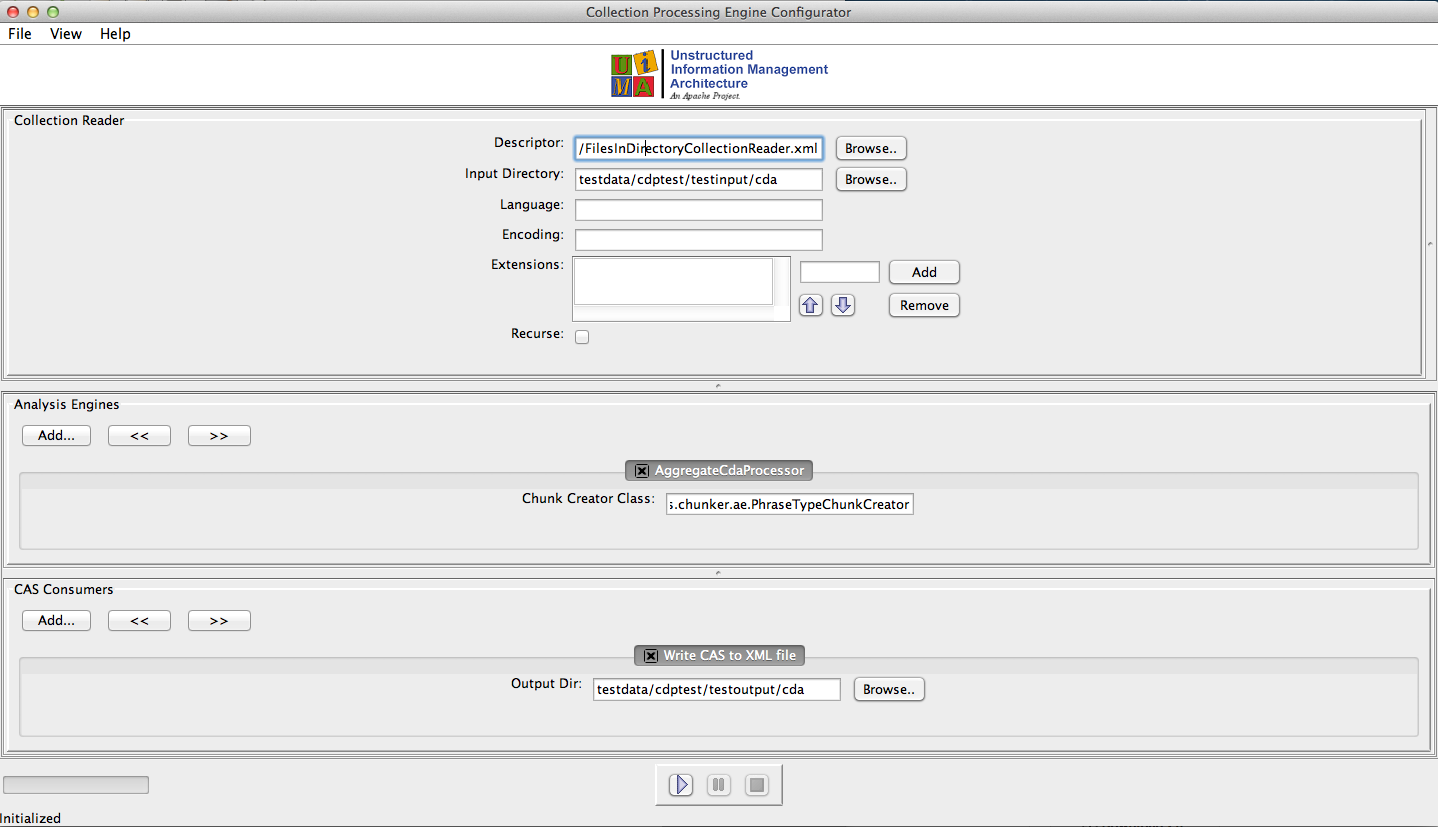
\includegraphics[scale=0.3]{ctakes.png}~  \\[1cm]

cTAKES provides instructions on how to batch process the files contained in the 'input' directory .
\\
medTurk uses cTAKES to process each clinical note for concepts and stores concepts according to three criteria.

\subsection*{Negation}
The first criteria is negation. The concept must have positive polarity, that is, it is not negated (e.g. the patient denies smoking).

\subsection*{Subject Analysis}
The second criteria is the concept must have a subject of patient. As an example, there are times when the a physician might write that a patient's father had lung cancer. In this example, the concept of "lung cancer" would have a subject of "Patient's Father". medTurk only extracts concepts which act directly on the patient.

\subsection*{Confidence}
The last criteria is confidence. cTAKES reports a confidence number for each extraction and medTurk only keeps concepts which have a confidence value of "1.0".



\section{Using medTurk}
To start up medTurk, ensure UMLS and MongoDB is running. Next, run the following script:

\begin{verbatim}
python run_server.py
\end{verbatim}
You should see something like the following:
\\
\\
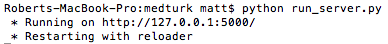
\includegraphics[scale=0.8]{run_server.png}~  \\[1cm]
Now, browse to the following URL in your browswer:

\begin{verbatim}
http://127.0.0.1:5000/medturk/index.html#/
\end{verbatim}

\subsection*{Home Page}
This is the landing page that contains a brief description of what medTurk is, and how to get started.

\subsection*{Create a Project Page}
To create a project, navigate to the project status page. You should see something like the following:

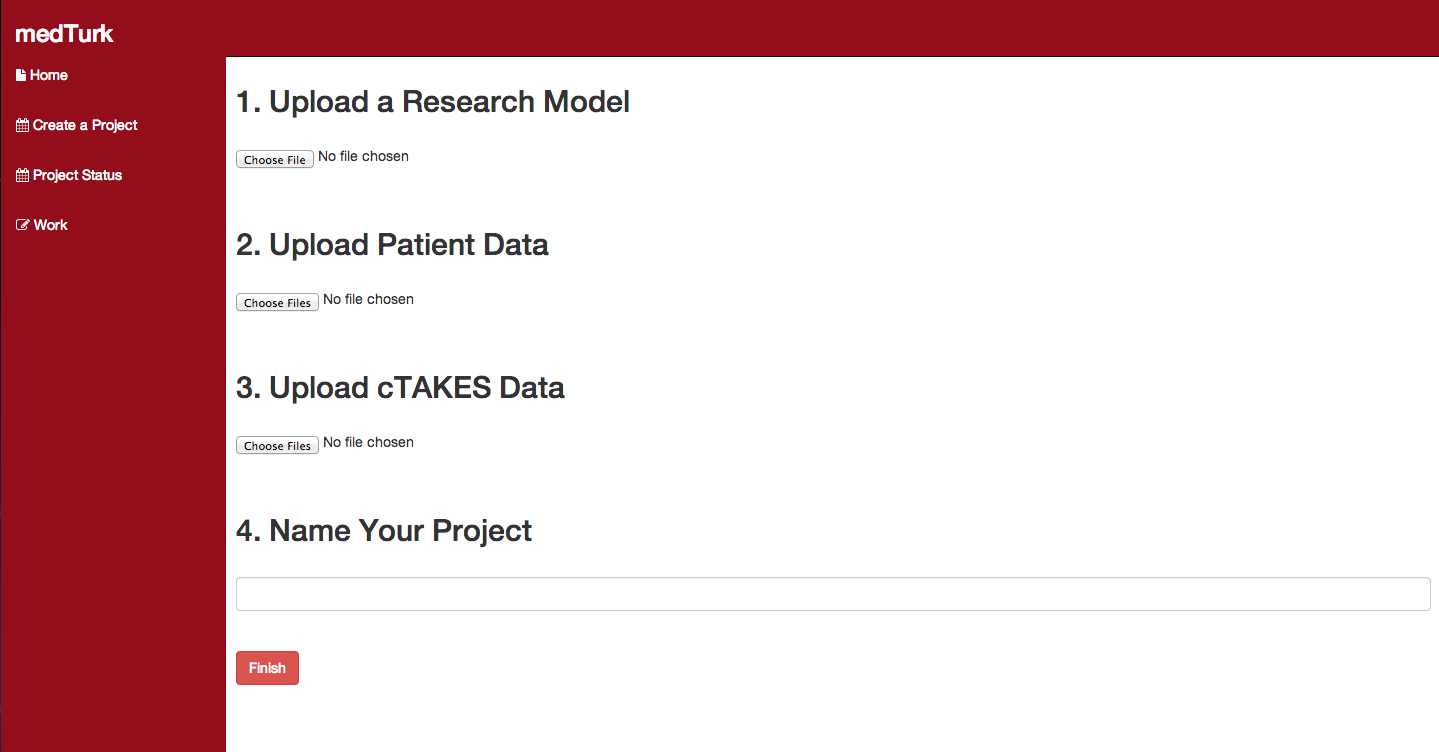
\includegraphics[scale=0.3]{create.png}~  \\[1cm]

\subsection*{Step 1}
Step 1 let's you upload your RM by navigating to it on your local computer. As an example, you may upload the late effects research model provided in medTurk found in:

\begin{verbatim}
medturk/models/late_effects.json
\end{verbatim}


\subsection*{Step 2}
Here, you can upload your one or more patient JSON files in the format explained in Section 3.1. As an example, you may upload the sample patient files found in:
\begin{verbatim}
medturk/example/patients/
\end{verbatim}


\subsection*{Step 3}
The Step 2, allows you to upload the processed cTAKES files. An an example, you may upload the sample cTAKES files found in:
\begin{verbatim}
medturk/example/ctakes/output/
\end{verbatim}

\subsection*{Step 4}
Here you may pick a name for your project. Click Finish and the project will be created.
\\
\section{Navigating medTurk}
medTurk contains four pages. This section briefly describes each page.

\subsection*{Project Status Page}
You may visualize the research model and view the percentage of project completion in the 'Project Status' page. This page also allows you to download answered questions in CSV format. This file can then be used for statistical analysis. 


\subsection*{Work Page}
You many answer questions by visiting this page. Each question provides clinical notes that are relevant to answering the question. 



\end{document}             % End of document.